\section{Background} 

Cutting-edge programmable NICs (named SmartNICs) rely their architectures either on (i) multi-threaded, multi-core flow processor units or (ii) on FPGAs (Field Programmable Gate Arrays) to meet the increasing and strict demand. We concentrate our analysis on the general architectural elements of the Netronome SmartNIC architecture~\cite{netronomeArc} -- which is used afterward in our performance experiments -- and rely on a multi-core architecture. 

\begin{figure}[!htb]
\centering
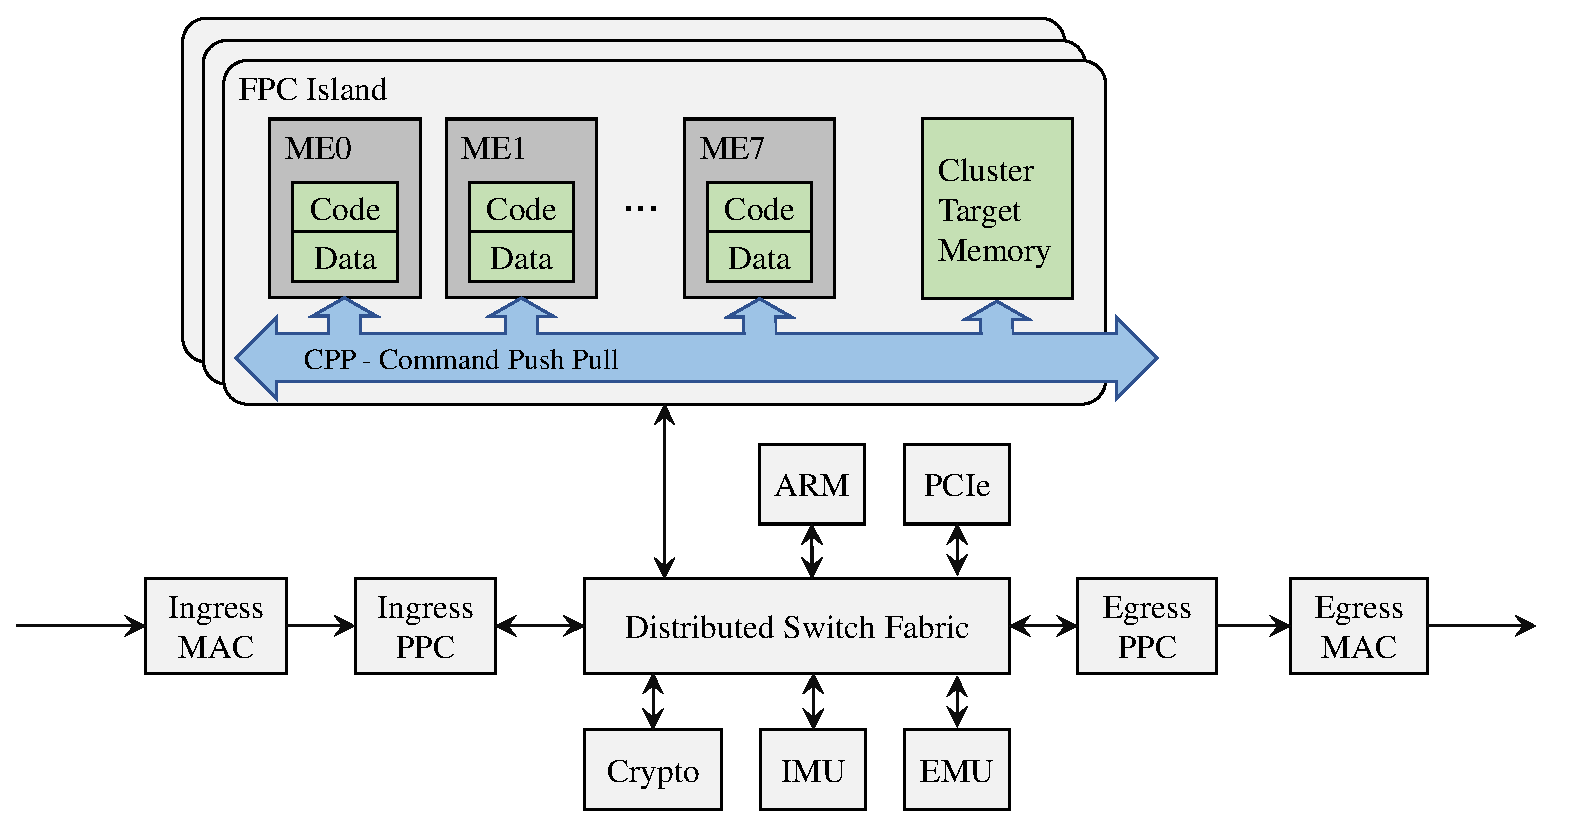
\includegraphics[scale=0.3]{img/architecture.eps}
\caption{An overview of the Netronome SmartNIC architecture~\cite{aina2021}.}
\label{fig-architecture}
\end{figure}

The SmartNIC Netronome NFP4000 architecture manages its flow processing cores (FPC) in multiple islands (Figure~\ref{fig-architecture}). Each FPC includes eight Micro Engines (MEs) as a particular processor keeping its own instruction store (\textit{code}) and local memory (\textit{data}). 
Therefore, every ME in the architecture can run code with all other MEs in parallel. To support this feature, each ME holds 8 threads that can be used for cooperative multithreading in the manner that,  at any given moment, at most, one thread is executing code from the same program. It means that each FPC handles at most eight parallel threads at 1.2Ghz (one thread per ME). In each FPC, local memory comprises 32-bit registers, shared between all eight threads. Such registers are separated into: (\textit{i}) general-purpose registers (256 32-bits registers) -- used by default to store any register of up to 32-bits size; (\textit{ii}) transfer registers (512 32-bits registers) -- used for copying register over the interconnection bus (e.g., from or to other FPCs or memories); (\textit{iii}) next-neighbor registers (128 32-bits registers) -- used mostly to intercommunicate with adjacent FPCs; and (\textit{iv}) local memory (1024 32-bit registers) -- which is a little bit slower than general register. When there is a demand for more memory than available space in local FPC registers, variables are automatically and statically assigned to other in-chip memory hierarchies. Further, there are other sorts of memory available to FPCs: (\textit{i}) Cluster Local Scratch (CLS) (20-50 cycles); (\textit{ii}) Cluster Target Memory (CTM) (50-100 cycles); (\textit{iii}) Internal Memory (IMEM) (120-250 cycles); and (\textit{iv}) External Memory (EMEM) (150-590 cycles). For further details, the interested reader is referred to~\cite{netronomeArc}. 

As packets are acquired from the network, an FPC thread picks up the packets and processes them. Extra threads are assigned to new packets as they arrive. For example, the SmartNIC NFP-4000 supports up to 60 FPCs, which enables the process of up to 480 packets simultaneously. The SmartNIC allows to program it directly using Micro-C language (i.e., a subset of C language) or using high-level domain-specific languages such as P4~\cite{p4-ref}. The code is then compiled and statically assigned to a particular subset of FPC. 

%In resume, the local memory register is used for data used in every packet. The CLS is used for data required for most packets and small shared tables. The CTM is used for packet headers and management between other sub-systems. IMEM is used for packet bodies and medium-sized shared tables. Finally, EMEM is used for extensive shared tables. 




%old:
%The SmartNIC architecture is illustrated in Fig. \ref{fig-architecture}. It organizes its flow processing cores (FPC) in multiple islands. Each FPC runs at most 8-threads in parallel at 1.2Ghz. However, in-chip islands do not follow the same architectural design. For example, some islands may contain mostly FPC processing units. Others, in turn, may have fewer processing units but other functionalities such as PCIe interfaces or crypt sub-systems.
%
%The FPC is a 32-bit machine and, therefore, all of its internal registers and local memory are formed from 32-bit words. FPCs follow a Harvard Architecture and therefore code and data occupy different memories. Usually, 4K bytes are shared between all 8 threads for data and a reserved memory of 8K instructions for the coding store. Every thread on an FPC runs the same program, held in the single code store shared by all the threads.
%
%Local memory in each FPC  is composed of a set of 32-bit registers, shared between all 8 threads. These registers are divided into (i) general-purpose registers (256 32-bits register) -- used by default to store any register of up 32-bits size; (ii) transfer registers (512 32-bits registers) -- used for copying register over the interconnection bus (e.g., from or to other FPCs or memories); (iii) next-neighbor registers (128 32-bits register) -- used mainly to communicate with neighboring FPCs; and last (iv) local memory (1024 32-bit register) -- which is a little bit slower than general register (3 cycles access, instead of just 1 cycle). When there is a need for more memory than available space in local FPC registers, variables are automatically and statically allocated to other in-chip memories hierarchies. 
%
%There are four other kinds of memory which are available to FPCs: (i) Cluster Local Scratch (CLS) (20-50 cycles); (ii) Cluster Target Memory (CTM) (50-100 cycles); (iii) Internal Memory (IMEM) (120-250 cycles); and (iv) External Memory (EMEM) (150-590 cycles). In summary, the local memory register is used for data that is used for every packet. Then, the CLS is used for data that is needed for most packets and small shared tables. The CTM is used for packet headers and coordination between other sub-systems. Then, IMEM is used for packet bodies and medium-sized shared tables. Finally, EMEM is used for large shared tables. 

%As packets are received from the network, an FPC thread picks up the packet and processes it. Additional threads are allocated to new packets as they arrive. For instance, the SmartNIC NFP-4000 supports up to 60 FPCs, each supporting up to 8 threads. Then, the device can process up to 480 packets simultaneously.


%Transfer registers. All data traveling over the CPP bus to or from CLS, CTM, IMEM, or EMEM must go through a transfer register. Just to emphasize this: CPP data cannot come directly from or go directly to general-purpose registers. It must instead go via transfer registers. There are 256 32-bit transfer-in registers, also known as “read registers”. These are used to receive data that arrives via a CPP Push operation. Several sequential registers can be transferred from the CPP bus in one Push operation. From ME code, these registers are read-only. They are shared between the 8 threads, so each thread has 32 transfer-in registers. There are also 256 32-bit transfer-out registers, also known as “write registers”. These are used to provide the data which is taken by a CPP Pull operation. Data from several sequential registers can be transferred onto the CPP bus in one Pull operation. From ME code, these registers are write-only. They are shared between the 8 threads, so each thread has 32 transfer-out registers. Transfer registers can in principle be indexed, but the ME hardware has only one transfer index register, shared between all threads, which makes generating code to use this index register slightly tricky. The compiler does not currently attempt to do this, and arrays that are indexed by values that vary at runtime cannot, therefore, be allocated to transfer registers.
%






